\documentclass[11pt]{article}

% -------------- PREÁMBULO ---------------

\usepackage[spanish]{babel} 
\usepackage[utf8]{inputenc} 
\usepackage{amsmath}
\usepackage{amssymb} 
\usepackage{graphicx}           % Incluir imágenes en LaTeX
\usepackage{color}              % Para colorear texto
\usepackage{subfigure}          % subfiguras
\usepackage{float}              % Podemos usar el especificador [H] en las figuras para que se queden donde queramos
\usepackage{capt-of}            % Permite usar etiquetas fuera de elementos flotantes (etiquetas de figuras)
\usepackage{sidecap}            % Para poner el texto de las imágenes al lado
\sidecaptionvpos{figure}{c}     % Para que el texto se alinee al centro vertical
\usepackage{caption}            % Para poder quitar numeracion de figuras
\usepackage{anysize}            % Para personalizar el ancho de  los márgenes
\marginsize{2cm}{2cm}{2cm}{2cm} % Izquierda, derecha, arriba, abajo
\usepackage{multicol}
\usepackage{multirow}
\setlength{\columnsep}{1cm}

% Para agregar encabezado y pie de página
\usepackage{fancyhdr} 

\usepackage{listings}
\pagestyle{fancy}
\fancyhf{}
\fancyhead[L]{\footnotesize USB}                  % Encabezado izquierda
\fancyhead[R]{\footnotesize Análisis de algoritmos}  
\fancyfoot[R]{\footnotesize Reporte}              % Pie derecha
\fancyfoot[C]{\thepage}                           % centro
\fancyfoot[L]{\footnotesize Ingeniería de la Computación}  %izquierda
\renewcommand{\footrulewidth}{0.4pt}

\newcommand{\coment}[1]{}
\definecolor{BurntOrange}{RGB}{247,148,42}

\begin{document}

% ----------------- PORTADA -----------------

\begin{center} 
   \newcommand{\HRule}{\rule{\linewidth}{0.5mm}}  

   \begin{minipage}{0.48\textwidth}
      \begin{center}
         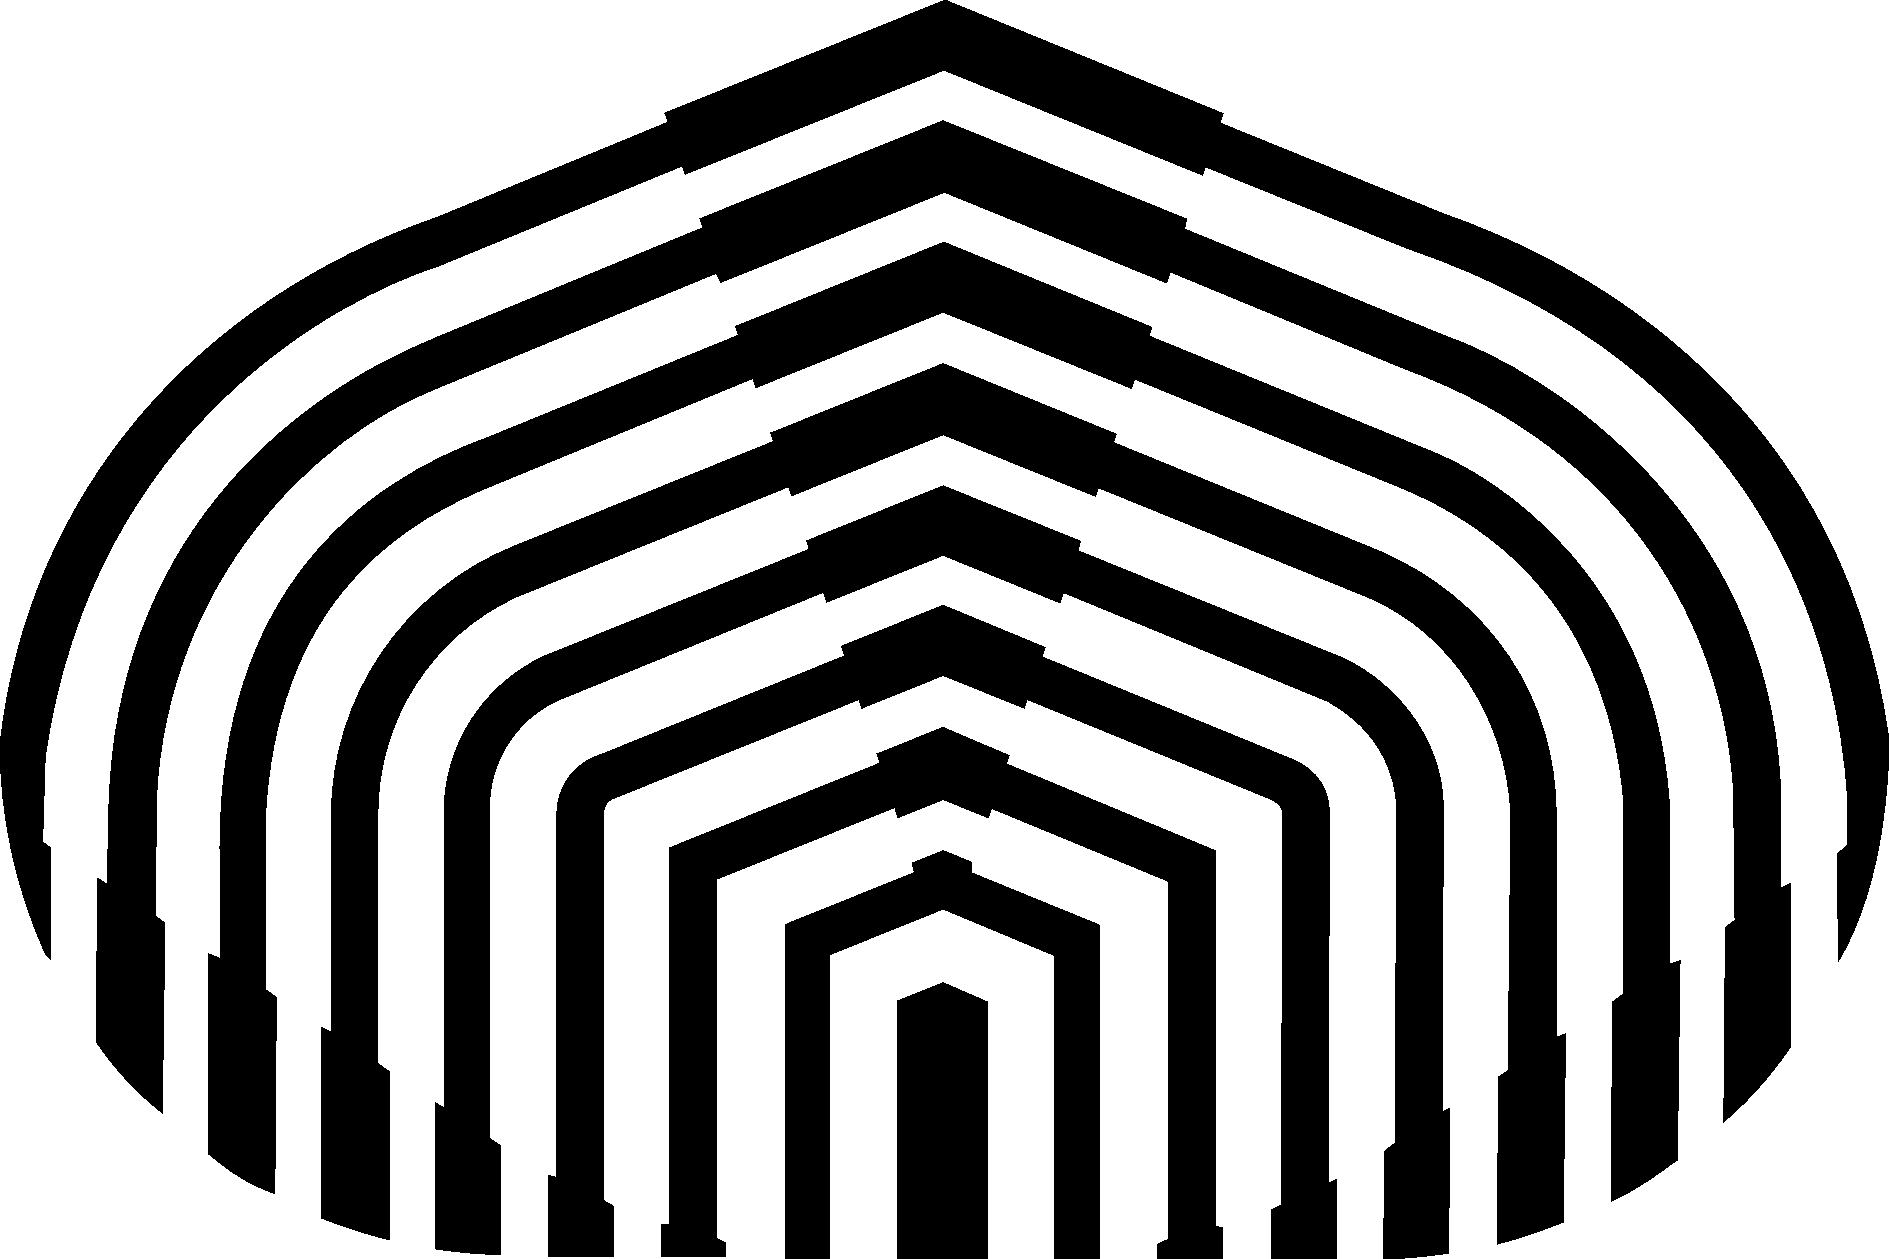
\includegraphics[scale = 0.5]{logo.png}
      \end{center}
   \end{minipage}

   \vspace*{1.0cm}                       
   \textsc{\huge Universidad Simón \\ \vspace{5px} Bolívar} \\ [1.5cm] 

   \begin{minipage}{0.9\textwidth} 
      \begin{center}                                                             
         \textsc{\LARGE Reporte de Laboratorio de Semana 5 }
      \end{center}
   \end{minipage} \\ [3cm]

   \vspace*{1cm}                                                                              
   \HRule \\ [0.4cm]                                                  
   {\huge \bfseries Análisis de algoritmos sobre grafos} \\ [0.4cm] 
   \HRule \\ [4cm]

   \begin{minipage}{\textwidth} 
      \begin{flushleft} \large    
         \textbf{\underline{Autor:}} \\ 
         Christopher Gómez \\
      \end{flushleft}
   \end{minipage}

   \begin{minipage}{\textwidth}    
      \vspace{-0.6cm}  
      \begin{flushright} \large    
         \textbf{\underline{Profesor:}} \\  
         Eduardo Blanco  
      \end{flushright}        
   \end{minipage} 

   \vspace*{1cm}
   \flushleft{\textbf{\Large Laboratorio de Algoritmos y Estructuras de Datos III (CI2693)} }\\
   \vspace{2cm}  

   \begin{center} 
      {\large \today} 
   \end{center}     
\end{center}                                                      
                                                               
\newpage
                                                    
% -------------------------------------------

\section{Metodología}

El siguiente estudio experimental consiste en correr un conjunto de algoritmos
sobre grafos no dirigidos para la búsqueda de componentes conexas y árboles mínimos
cobertores sobre tres grafos de prueba de distinto número de vértices y lados,
midiendo sus tiempos de ejecución y tomando nota de los resultados. \\

Solamente se toma el tiempo de ejecución del algoritmo. \\

Los algoritmos a ejecutar, implementados en el lenguaje de programación Kotlin,
serán los siguientes: 

\begin{itemize}
   \item \textbf{Algoritmos para hallar componentes conexas}:
   \begin{itemize}
      \item Basado en la estructura de conjuntos disjuntos.
      \item Basado en el algoritmo de Búsqueda en Profundidad.
   \end{itemize}
   \item \textbf{Algoritmos para hallar árboles mínimos cobertores}:
   \begin{itemize}
      \item Algoritmo de Kruskal (usando en la estructura de conjuntos disjuntos).
      \item Algoritmo de Prim (usando una cola de prioridad basada en un heap binario).
   \end{itemize}
\end{itemize}

Los siguientes son los detalles de la máquina y el entorno donde se ejecutaron los algoritmos:

\begin{itemize}
   \item \textbf{Sistema operativo}: Debian 11 Bullseye 64-bit.
   \item \textbf{Procesador}: Intel(R) Core(TM) i3-2120 CPU @ 3.30GHz.
   \item \textbf{Memoria RAM}: 4,00 GB (3, 88 GB usables).
   \item \textbf{Compilador}: kotlinc-jvm 1.5.31 (JRE 11.0.12+7-post-Debian-2).
   \item \textbf{Entorno de ejecución}: OpenJDK Runtime Environment (build 11.0.12+7-post-Debian-2).
   \item \textbf{Flags (máquina virtual)}: -Xmx2g.
\end{itemize}

\section{Resultados experimentales}

\subsection{Algoritmos para hallar componentes conexas}

Los Cuadros 1 y 2 muestran los resultados obtenidos de aplicar los algoritmos
para hallar componentes conexas sobre los grafos de prueba. \\

Como se puede observar em el Cuadro 1, ambos algoritmos muestran los mismos resultados
al momento de hallar componentes conexas de un grafo no dirigido, lo cual 
nos indica que, a pesar de diferir en su funcionamiento, son equivalentes y dan 
el resultado correcto. \\

\newpage

% Primera tabla: Algoritmos para hallar componentes conexas
\begin{table}[t]
   \centering
   \begin{tabular}{lcc}
      \hline
      \textbf{Archivo} & \multicolumn{1}{l}{\textbf{Conjuntos disjuntos}} & \multicolumn{1}{l}{\textbf{Búsqueda en Profundidad}} \\ \hline
      \texttt{pequenio.txt} & 3 & 3 \\
      \texttt{mediano.txt} & 1 & 1 \\
      \texttt{grande.txt} & 1 & - \\ \hline
   \end{tabular}
   \label{tab:componentes}
   \caption{Número de componentes conexas detectadas según cada algoritmo.}
   \vspace{-1em}
\end{table}


% Segunda tabla: Tiempo de ejecución de componentes conexas
\begin{table}[t]
   \centering
   \begin{tabular}{lcc}
      \hline
      & \multicolumn{2}{c}{\textbf{Tiempo (ms)}}   \\ \hline
      \textbf{Archivo} & \multicolumn{1}{c}{\textbf{Conjuntos disjuntos}} & \multicolumn{1}{c}{\textbf{Búsqueda en Profundidad}} \\ \hline
      \texttt{pequenio.txt} & 8 & 1 \\
      \texttt{mediano.txt} & 15 & 2 \\
      \texttt{grande.txt} &  9423 & - \\ \hline
   \end{tabular}
   \label{tab:tiemposcc}
   \caption{Tiempo de ejecución de los algoritmos para hallar componentes conexas.}
\end{table}


Por otro lado, es notorio observando el Cuadro 2 que el algoritmo basado en Búsqueda 
en Profundidad se ejecuta considerablemente más rápido que el basado en la
estructura de Conjuntos Disjuntos para los archivos \texttt{pequenio.txt} y
\texttt{mediano.txt}, sin embargo, para el archivo \texttt{grande.txt} se obtuvo
un resultado singular, y es que mientras el algoritmo basado en Conjuntos Disjuntos
se ejecutó en un tiempo de 12,8s aproximadamente, el algoritmo basado en Búsqueda en
Profundidad arroja el siguiente error de memoria antes de terminar de ejecutarse, por lo que 
no se obtienen resultados: \\

\begin{lstlisting}
Exception in thread "main" java.lang.StackOverflowError
   at ve.usb.grafoLib.GrafoNoDirigido.adyacentes(GrafoNoDirigido.kt:142)
   at ve.usb.grafoLib.ComponentesConexasDFS.dfsVisit(ComponentesConexasDFS.kt:52)
   at ve.usb.grafoLib.ComponentesConexasDFS.dfsVisit(ComponentesConexasDFS.kt:57)
   at ve.usb.grafoLib.ComponentesConexasDFS.dfsVisit(ComponentesConexasDFS.kt:57)
                                    .
                                    .
                                    .
\end{lstlisting}

La razón de que esto ocurra en el archivo \texttt{grande.txt} es que este contiene un
grafo de un millón de vértices y más de siete millones de aristas, y además, como
se observa en el resultado dado por el otro algoritmo, que el grafo tiene una sola
componente conexa, lo cual implica que la búsqueda profunda puede necesitar mantener
más de $3$ mil llamadas recursivas\footnote{Cifra tomada de una prueba que no se halla en el código fuente adjunto, en
la que se cuentan la cantidad de llamadas recursivas que se mantienen en la ejecución 
del algoritmo. El resultado mostró 3336 llamadas empiladas antes de lanzar error por
desbordamiento de pila.} para transversar determinados caminos en el grafo,
causando rápidamente\footnote{En menos de 2s. según mediciones con herramientas externas}
un desbordamiento de la pila (con la configuración referida
en la sección 1). \\

Salvo por esta excepción, los resultados obtenidos para estos algoritmos concuerdan con
la teoría, de la cual podemos deducir que el algoritmo basado en Conjuntos Disjuntos,
usando las heurísticas de compresión de camino y de unión por rango, tienen un tiempo
de ejecución de $O((|V|+||E)\alpha(|V|))$ (donde $\alpha(|V|)$ es una constante menor a
4), ya que involucra $|V| + |E|$ operaciones de \texttt{Make-Set}, \texttt{Find-Set} y 
\texttt{Union}, de las cuales $|V|$ son \texttt{Make-Set}. Por otra parte, el tiempo de 
ejecución del algoritmo basado en DFS es de solo $O(|V|+|E|)$, lo cual indica que las 
constantes involucradas en el otro algoritmo hacen una diferencia notoria en la práctica. \\

A raíz de estas últimas pruebas, se decidió adicionalmente implementar una versión iterativa
de la Búsqueda en Profundidad, evitando las llamadas recursivas de \texttt{DFS-Visit} mediante
una pila de vértices. Los resultados se recogen en el Cuadro 3, y del mismo podemos ver que,
a pesar de obtener unos resultados similares a los de la versión recursiva para los mismos
archivos de prueba, esta vez sí se logra terminar la ejecución y el tiempo para \texttt{grande.txt}
es más de $8$ veces menor al resultado para el algoritmo de Conjuntos Disjuntos, lo cual 
deja en evidencia la eficiencia del algoritmo.

\begin{table}[t]
   \centering
   \begin{tabular}{lcc}
      \hline
      \textbf{Archivo} & \multicolumn{2}{c}{\textbf{Tiempo (ms)}}   \\ \hline
      \texttt{pequenio.txt} & 0 \\
      \texttt{mediano.txt} & 3 \\
      \texttt{grande.txt} & 1164 \\ \hline
   \end{tabular}
   \label{tab:tiemposccit}
   \caption{Tiempo de ejecución del DFS Iterativo para hallar componentes conexas.}
\end{table}

\subsection{Algoritmos para hallar árboles mínimos cobertores}

En los Cuadros 4 y 5 se muestran los resultados de ejecutar los algoritmos de Kruskal
y Prim sobre los archivos dados. \\


% Cuarta tabla: Peso del árbol mínimo cobertor hallada según cada algoritmo
\begin{table}[h]
   \centering
   \begin{tabular}{lcc}
      \hline
      \textbf{Archivo} & \multicolumn{1}{c}{\textbf{Kruskal}} & \multicolumn{1}{c}{\textbf{Prim}} \\ \hline
      \texttt{gnd-pequenio.txt} & 1.81 & 1.8099999999999998 \\
      \texttt{gnd-mediano.txt} & 10.463510000000001 & 10.463509999999994 \\
      \texttt{gnd-grande.txt} & 647.6630695500033 & 647.6630695499884 \\ \hline
   \end{tabular}
   \label{tab:pesos}
   \caption{Peso calculado del árbol mínimo cobertor hallado según cada algoritmo.}
\end{table}

% Cuarta tabla: Tiempo de ejecución de árboles mínimos cobertores
\begin{table}[h]
   \centering
   \begin{tabular}{lcc}
      \hline
      & \multicolumn{2}{c}{\textbf{Tiempo (ms)}}   \\ \hline
      \textbf{Archivo} & \multicolumn{1}{c}{\textbf{Kruskal}} & \multicolumn{1}{c}{\textbf{Prim}} \\ \hline
      \texttt{gnd-pequenio.txt} & 22 & 2 \\
      \texttt{gnd-mediano.txt} & 34 & 9 \\
      \texttt{gnd-grande.txt} &  21016 & 5762 \\ \hline
   \end{tabular}
   \label{tab:tiemposamc}
   \caption{Tiempo de ejecución de los algoritmos para hallar árboles mínimos cobertores.}
\end{table}

Los resultados obtenidos muestran que en todos los casos el algoritmo de Prim es 
más eficiente que la implementación del algoritmo de Kruskal usando Conjuntos Disjuntos.
Como se puede observar en el Cuadro 4, ambos algoritmos hallan árboles mínimos cobertores
con pesos muy parecidos, lo cual verifica que en ciertos casos tanto el algoritmo de Prim
como el de Kruskal, a pesar de funcionar de forma distinta, hallan el mismo árbol mínimo
cobertor. Aunque no se verificó para los archivos \texttt{gnd-mediano.txt} y \texttt{gnd-grande.txt},
para \texttt{gnd-pequenio.txt}, efectivamente, los árboles mínimos cobertores son idénticos,
sin embargo, el cálculo del peso da una diferencia de $2*10^{-17}$ entre Kruskal y Prim, lo
cual puede deberse a que en cada arbol las aristas son agregadas en la lista de lados
en orden distinto, generando errores de redondeo en la aritmética de precisión finita que se efectúa
en el computador para operaciones de punto flotante al momento de sumar los pesos en distinto orden. \\

Por otro lado, para los árboles en \texttt{gnd-mediano.txt} y \texttt{gnd-grande.txt} no se 
puede asegurar si ambos árboles son exactamente los mismos y se trata nuevamente de errores
en la aritmética, o si son distintos árboles, pero sí se puede notar que tanto Kruskal como Prim
son capaces de dar resultados razonables, aunque para el caso de Prim dependa del vértice
que se escoja como fuente. \\

Tal como se enuncia en la teoría, los algoritmos con Conjuntos Disjuntos no suelen preferirse
por encima de otros algoritmos para resolver los mismos problemas. En este caso, aunque
tanto el algoritmo de Prim como el de Kruskal tienen teóricamente un tiempo
asintótico de $O(|E|log|V|)$, en la práctica podemos ver que que el algoritmo de Prim resulta
siempre alrededor de 4 veces más rápido, lo cual puede ser un indicativo de que las operaciones
sobre la estructura de Conjuntos Disjuntos pueden resultar más costosa que las operaciones
sobre heaps binarios, y que el procedimiento de ordenar las aristas por sus pesos
esconde constantes que en aplicaciones prácticas en necesario tener en cuenta.

\subsection{Conclusiones}

Finalmente, la implementación de estos algoritmos, los resultados obtenidos en las pruebas, y su
posterior análisis permiten obtener las siguientes conclusiones:

\begin{itemize}
   \item Aunque la estructura de Conjuntos Disjuntos es facil de implementar y es útil 
   para usar en algoritmos más sencillos de entender, generalmente suelen tener un peor 
   desempeño en la práctica.
   \item Los algoritmos recursivos pueden resultar más elegantes y fáciles de entender,
   sin embargp, en ciertos casos se puede presentar un número excesivo de llamadas recursivas,
   dando lugar a fallos en su funcionamiento, por lo que es recomendable cuidar los detalles
   de sus implementaciones o usar alguna variante iterativa si se sabe que el algoritmo
   será usado para propósitos que manejen instancias grandes de problemas y pocos recursos.
   \item La Búsqueda en Profundidad puede ser modificada para muchos propósitos distintos, además
   de el de encontrar caminos o marcar tiempos. 
   \item Algoritmos con la misma complejidad temporal pueden desempeñarse en la práctica 
   de forma muy distinta.
   \item Es recomendable implementar formas de evitar errores en la aritmética si es de suma
   importancia la precisión de los cálculos para los pesos de los AMC.
   \item Es importante asegurar la escalabilidad de las implementaciones que se hacen, pues a
   menudo las aplicaciones de la vida real involucran instancias de problemas gigantescas, y
   se necesita no perder eficiencia ni eficacia en los resultados. Asegurar la escalabilidad 
   requiere en algunos casos repensar los algoritmos o el funcionamiento de las estructuras que 
   este involucra, o hasta implementarlas y prescindir de librerías, para que se acoplen de la 
   mejor forma a las necesidades.
\end{itemize}

\end{document}